\documentclass[xetex,mathserif,serif]{beamer}
\usepackage{polyglossia}
\setdefaultlanguage[babelshorthands=true]{russian}
\usepackage{minted}
\usepackage{tabu}
\usepackage{moresize}

\useoutertheme{infolines}

\usepackage{fontspec}
\setmainfont{FreeSans}
\newfontfamily{\russianfonttt}{FreeSans}

\definecolor{links}{HTML}{2A1B81}
\hypersetup{colorlinks,linkcolor=,urlcolor=links}

\tabulinesep=1.2mm

\title{Коллекции из стандартной библиотеки Java}
\author[Юрий Литвинов]{Юрий Литвинов\\\small{\textcolor{gray}{yurii.litvinov@gmail.com}}}
\date{30.01.2019г}

\newcommand{\attribution}[1] {
\vspace{-5mm}\begin{flushright}\begin{scriptsize}\textcolor{gray}{\textcopyright\, #1}\end{scriptsize}\end{flushright}
}

\begin{document}

	\frame{\titlepage}

	\section{Коллекции}

	\begin{frame}
		\frametitle{Коллекции}
		\begin{itemize}
			\item Интерфейсы коллекций
			\item Реализации общего назначения
			\item Специализированные реализации
			\item Многопоточные реализации
			\item Абстрактные реализации
			\item Обёртки
			\item Алгоритмы
			\item Инфраструктура
		\end{itemize}
	\end{frame}

	\begin{frame}
		\frametitle{Основные интерфейсы}
		\begin{itemize}
			\item Iterable --- всё, по чему можно итерироваться
			\item Collection --- просто группа объектов
			\begin{itemize}
				\item Set, SortedSet --- множества
				\item List --- упорядоченная коллекция, вводит понятие ``позиция''
				\item Queue, Deque --- очереди, деки
			\end{itemize}
			\item Map --- отображение
			\begin{itemize}
				\item SortedMap
				\item NavigableMap --- позволяет получить элемент, ближайший к искомому
			\end{itemize}
		\end{itemize}
	\end{frame}

	\begin{frame}
		\frametitle{Реализации общего назначения}
		\begin{footnotesize}
			\begin{tabu} {| X[1 l p] | X[0.7 l p] | X[1 l p] | X[0.7 l p] | X[1 l p] | X[1.3 l p] |}
				\tabucline-
				Интерфейс  & Хеш-таблица  & Массив      & Дерево   & Список      & Хеш-таблица + Список  \\
				\tabucline-
				\everyrow{\tabucline-}
				Set        & HashSet      &             & TreeSet  &             & LinkedHashSet         \\
				List       &              & ArrayList   &          & LinkedList  &                       \\
				Deque      &              & ArrayDeque  &          & LinkedList  &                       \\
				Map        & HashMap      &             & TreeMap  &             & LinkedHashMap         \\
			\end{tabu}
		\end{footnotesize}
	\end{frame}

	\begin{frame}
		\frametitle{Абстрактные реализации}
		\begin{itemize}
			\item AbstractCollection
			\begin{itemize}
				\item Требуется iterator() с hasNext() и next() и size()
				\item Для возможности модификации --- переопределить add() и, для итератора, remove()
				\item Надо конструктор без аргументов и принимающий Collection
				\item Могут быть переопределены остальные методы, для большей эффективности
			\end{itemize}
			\item AbstractSet
			\item AbstractList
			\item AbstractSequentialList
			\item AbstractMap
			\begin{itemize}
				\item Требуется реализовать entrySet()
				\begin{itemize}
					\item ``View Collection'' --- сам элементы не хранит
				\end{itemize}
				\item Для возможности модификации --- переопределить put() и, для итератора, remove()
			\end{itemize}
		\end{itemize}
	\end{frame}

	\begin{frame}
		\frametitle{Инфраструктура}
		\begin{itemize}
			\item Iterator
			\begin{itemize}
				\item hasNext()
				\item next()
				\item remove() --- можно не реализовывать
			\end{itemize}
			\item ListIterator --- двунаправленный, работает с индексами
			\item Comparable --- задаёт Natural Ordering
			\item Comparator --- задаёт произвольный порядок
		\end{itemize}
	\end{frame}

	\begin{frame}
		\frametitle{Диаграмма}
		\begin{center}
			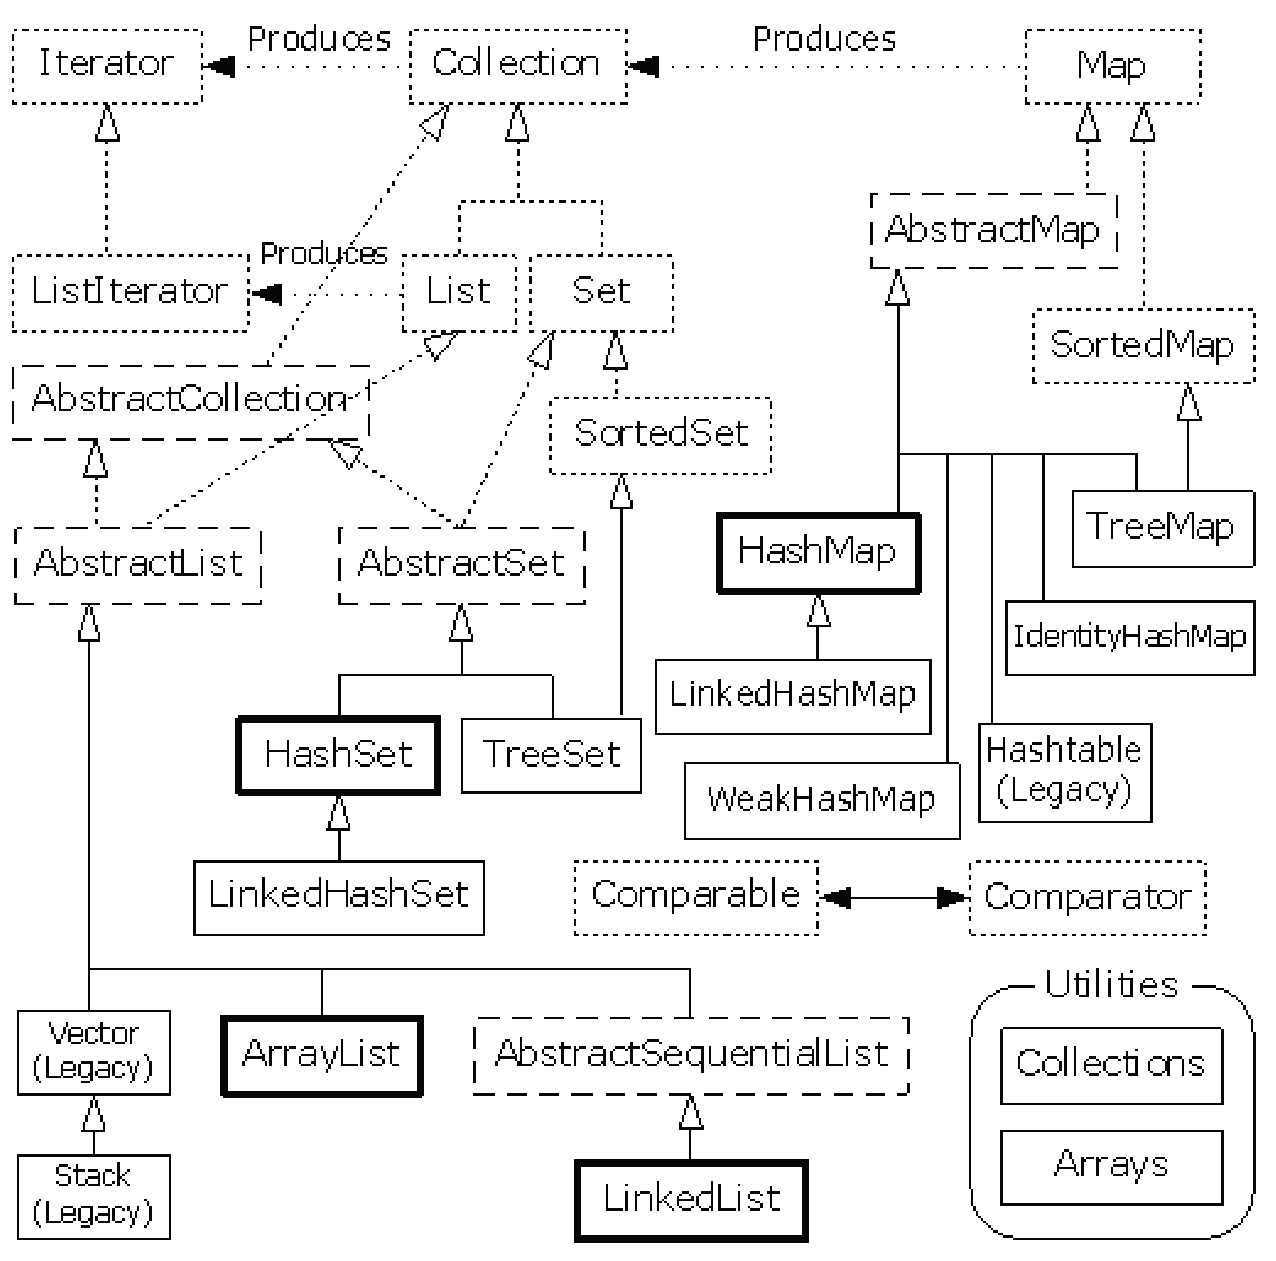
\includegraphics[width=0.6\textwidth]{java4Containers.png}
			\attribution{B. Eckel, Thinking in Java}
		\end{center}
	\end{frame}

	\begin{frame}
		\frametitle{Исключения}
		\begin{itemize}
			\item UnsupportedOperationException --- реализация не поддерживает метод, объявленный в интерфейсе (помечен как optional)
			\item ConcurrentModificationException --- попытка продолжить обход изменившейся коллекции
		\end{itemize}
	\end{frame}

	\begin{frame}
		\frametitle{Утилиты}
		\begin{itemize}
			\item java.util.Collections
			\begin{itemize}
				\item binarySearch, copy, sort, shuffle и т.д.
				\item emptyList, emptyMap, ...
				\item singleton, singletonList, ...
				\item unmodifiableList, unmodifiableMap, ...
			\end{itemize}
			\item java.util.Arrays
			\begin{itemize}
				\item asList
				\item sort, compare, equals, fill и т.д. для разных примитивных типов
			\end{itemize}
		\end{itemize}
	\end{frame}

	\section{Задача}

	\begin{frame}
		\frametitle{Задача}
		Переделать список из задачи про хеш-таблицы, чтобы он был генериком и реализовывал стандартный интерфейс \mintinline{java}|List<E>|. Нужны:
		\begin{itemize}
			\item Мутабельность
			\item Более эффективный итератор, чем по умолчанию
			\begin{itemize}
				\item С remove()
			\end{itemize}
			\item Эффективный ListIterator
			\item Тесты
		\end{itemize}
	\end{frame}

\end{document}
